\subsection{Chemical pre-processor [{\color{red}3 pages, Dennis and Mickelson}]}\label{sec:chempreproc}

The first task was to generate the proper code to optimize.  This involved finding a version of CESM, along with a model configuration and resolution that was able to run both the scalar and vectorized versions of the code generated by the chemistry preprocessor.  CESM model version cesm1\_4\_alpha07c was chosen with model configuration FWTC4L40CCMIR1 at 2 degree resolution (FV 1.9x2.5).  This model configuration uses WACCM with Troposphere, Stratosphere, Mesosphere, and Lower Thermosphere (TSMLT) chemistry.  The CESM/CMIP6 atmospheric chemistry runs will also include the Modal Aerosol Model 4 (MAM).  This configuration was not used for this project because the code was still in flux and was not ready in time for this project.  Because our goal was to optimize the chemistry preprocessor, our hope was that the optimizations we did at the tested configuration will be able to optimize all chemistry code generated by the tool.

After a stable chemistry configuration was found, we generated a KGEN kernel [6].  KGEN allowed us to create a standalone-testing kernel.  Once configured, it captured the Fortran code and the input and output arguments needed to run this section of the code.  It also incorporated a testing environment that allowed us to test different optimizations and test to see if the answers were changed.  This allowed us to experiment with different optimization techniques without the need of running CESM and provided a quicker turn around.

Two KGEN kernels were generated, one for the original scalar version and one for the vectorized version.  The versions of the code were checked into a GitHub repository and code optimization work was checked into the repository as branches.

It is also important to get better results on Intel?s Haswell and KNC processors.  The Haswell processor is similar to the Broadwell processor that will be installed into NCAR?s next production machine, Cheyenne [3].  CESM will also be expected to run efficiently on the Knights Landing (KNL) processor.  This will be important as Cori Phase II goes into production at NERSC with KNL processors.  

The first step was to get base timings for both the scalar and vector versions of the kernel.  During this process it was discovered that the answers changed in both the scalar and vector version when the code was ran on the Haswell and KNC.  It was found that the Fused Multiply-Add (FMA) instruction set was causing the answers to differ.  The answers matched when the code was built with the ?-no-fma? compiler flag.  Since it was important to track if any of the optimization work changed answers, this flag was used in all builds.  The base timings without optimizations are shown rows 1 and 2 in Table 2.  The out of the box vector code out performed the scalar version on Sandy Bridge, but took longer to run on the other two architectures.

Our next step was to understand the code better and to determine how the code was or was not being optimized.  This was done by building with the compiler flag ?-qopt-report=5? and by running with Intel Advisor [7].  Intel Advisor is a profiling tool that is able to evaluate a code?s performance.   It is able to inform the user why performance is poor and provides suggestions on how to improve the performance.  Both Intel Advisor and the optimization report stated that the compiler was performing no vectorization.  This was because several of the array sizes were declared dynamically.  Since the compiler did not know the sizes of the arrays, it did not know how to vectorize them.

In order to force the code to vectorize, we needed to declare the array sizes correctly.  This was done by removing the dynamic declarations and by replacing them with the variable sizes.  Code vectorization by the compiler was then confirmed within the optimization reports.  The timing results are shown in row 3 in Table 2 (?Vector w/ Better Declarations?).  This improved the speedup on Sandy Bridge by 1.38 and on Haswell by 1.35 over the original scalar kernel.  This improved the KNC performance by reducing the time to ? of the original vector time, though better performance was still seen in the KNC scalar code.

Once the code was vectorized, our attention turned to improving the memory usage.  As a simple test, we decided to modify the vector length.  The original vector length had been set to 13 to match the number of columns in the model.  The code then looped in groups of 13 until the total number of points, 858, was solved for.  858 is the total number of columns (13) times the number of levels (66).  As a test, we decided to set the vector length to 858, the total for this loop.  The timing results are in row 4 in Table 2 (?Vector w/ Vector Length = total \# of points?).  While this provided us with performance improvement across all three architectures, it also increased the cache misses because of it?s larger memory footprint.

\input chem-timing.tex 

In order to try to reduce the memory footprint, we tried adding ?Distribute\_Point? directives to the file mo\_lu\_factor.F90, the most time consuming portion of the code.  The DISTRIBUTE\_POINT directive is used to divide up a large ?DO? loop into several smaller loops.  When it is placed above the loop, the compiler tries to determine how to break up the loop.  Placing the directive inside the loop forces the compiler to break the loop at that point [8].  The file, mo\_lu\_factor.F90,  consists of twenty subroutines, each having one ?DO? loop that ranges in size from 100-600 lines.  As a starting point, the directives were added every five lines within the loops.  The results are shown in row 5 in Table 2 (?Vector w/ Distribute\_Point to break up loops?).  This increased the performance by about 0.1 on Sandy Bridge and Haswell and by about 0.01 on KNC.  

%\begin{figure}[tbp]
% \begin{center}
%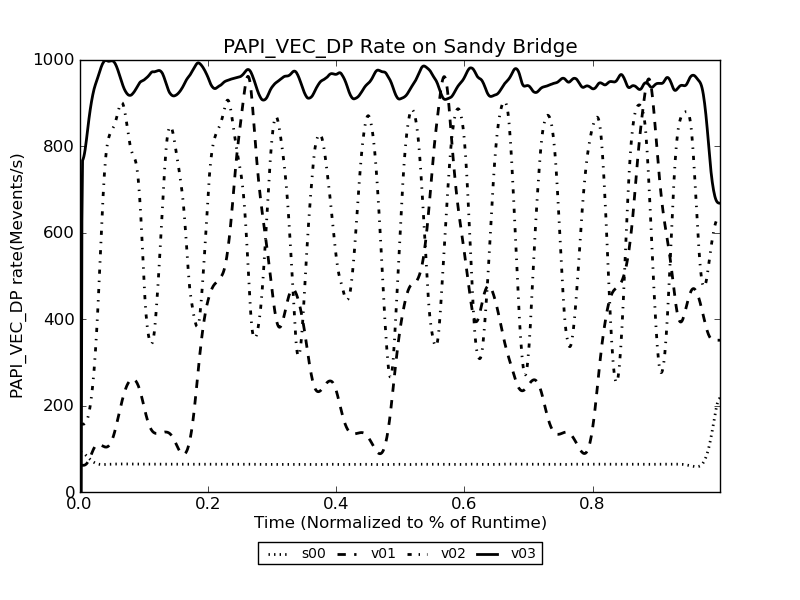
\includegraphics[width=12.0cm]{figures/PAPI_VEC_DP.png}
%\end{center}
%\caption{A plot of the fraction vector instructions on Haswell for several different versions of the implicit chemistry solver. }
%\label{fig:chem-vec-dp}
%\end{figure}

We next wanted to try reducing the memory footprint through cache blocking.  The easiest way to do this was to adjust the vector length variable.  As discussed earlier, the original value was 13 (the number of model columns) and it had been changed to 858 (the number of columns times the number of levels) during optimization testing.  We believed this larger memory footprint would be an issue as we scaled from 1 rank per node to 16 on Sandy Bridge and 72 on Haswell.  The red bars in Figures 1 and 2 confirmed this.  As the number of tasks was increased on a rank, it took longer to run because we were running out of space in cache.  In both cases, the vector time took longer than the scalar time (the blue bars in Figures 1 and 2) when it was fully scaled, causing us to loose all of our previous optimization work.  

%\begin{figure}[tbp]
% \begin{center}
%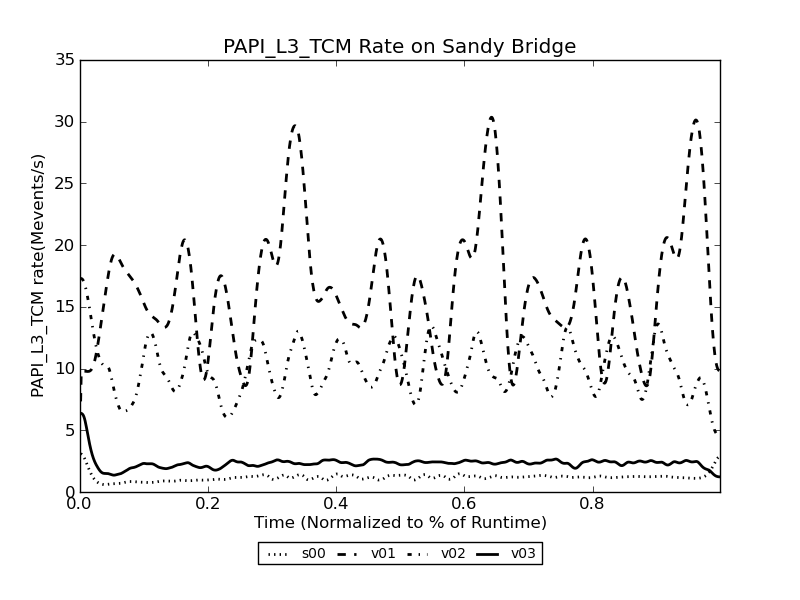
\includegraphics[width=12.0cm]{figures/PAPI_L3_TCM.png}
%\end{center}
%\caption{A plot of the total L3 cache miss rates on Haswell for several different versions of the implicit chemistry solver. }
%\label{fig:chem-l3-tcm}
%\end{figure}


In order to find the optimal value, we devised an experiment where the large arrays were systematically halved until our run times were not increasing with MPI task counts.  This allowed us to find the largest size that would fit into memory and scale across the all cores.  Through testing, we found that the optimal value was a vector length of 64 on Sandy Bridge.  The improvements for both Sandy Bridge and Haswell are shown in the green bars in Figures 1 and 2.  It was noted that the scaling on Sandy Bridge was slightly better than what was seen on Haswell.  At full scale, the speedup over the scalar version was 1.92 on Sandy Bridge and 1.36 on Haswell.  A separate test of a vector length of 32 was performed on Haswell, which yielded a speedup of 1.58 over the scalar version.  This will have to be studied further to determine if the different architectures require different vector lengths or if there is another cause for this.

\begin{figure}[tbp]
 \begin{center}
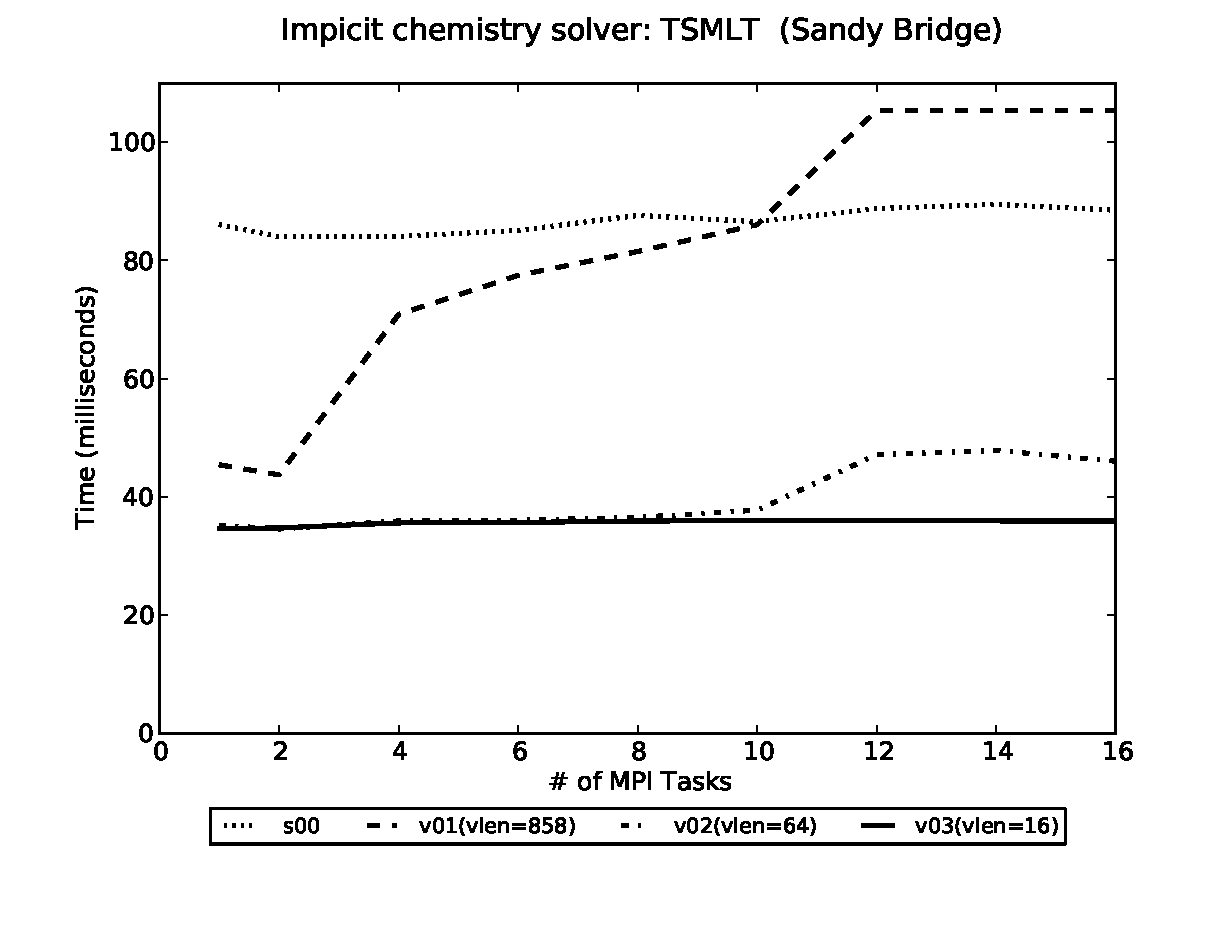
\includegraphics[width=12.0cm]{figures/chem-snb.pdf}
\end{center}
\caption{Weak scaling of several different versions of the implicit chemistry solver on Sandybridge {\color{red} FIXME: v03 data is missing. Color not allowed in book.}}
\label{fig:chem-weak-snb}
\end{figure}

\begin{figure}[tbp]
 \begin{center}
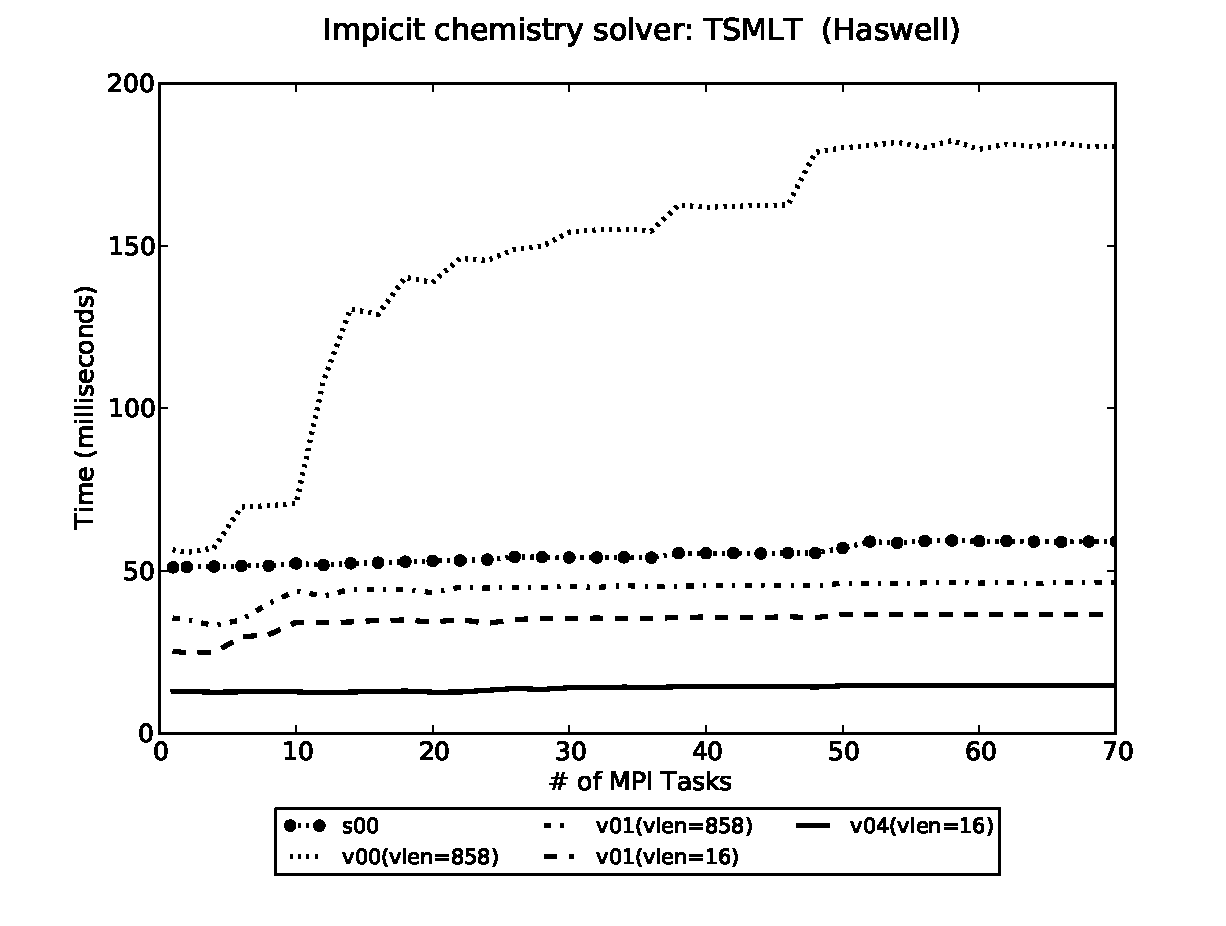
\includegraphics[width=12.0cm]{figures/chem-hsw.pdf}
\end{center}
\caption{Weak scaling of several different versions of the implicit chemistry solver on Haswell. {\color{red} FIXME:  v03 data is missing. Color not allowed in book.}}
\label{fig:chem-weak-haswell}
\end{figure}


\begin{figure}[tbp]
\begin{minipage}{1.\textwidth}
     \begin{center}
      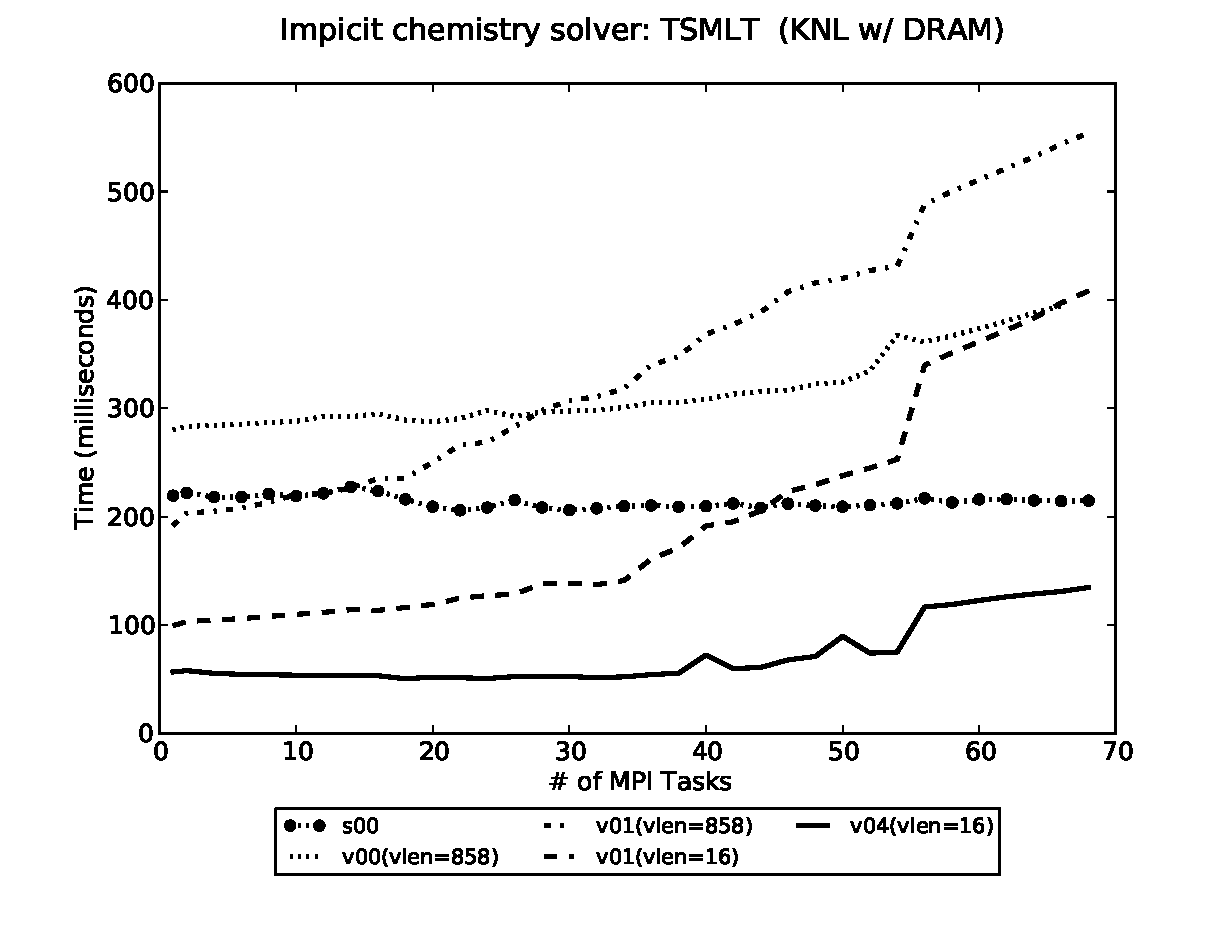
\includegraphics[width=12.0cm]{figures/chem-knl-dram.pdf}
      \caption{Weak scaling for the implicit chemistry solver Knights Landing using DRAM}
      \end{center}
\end{minipage}
\begin{minipage}{1.\textwidth}
     \begin{center}
      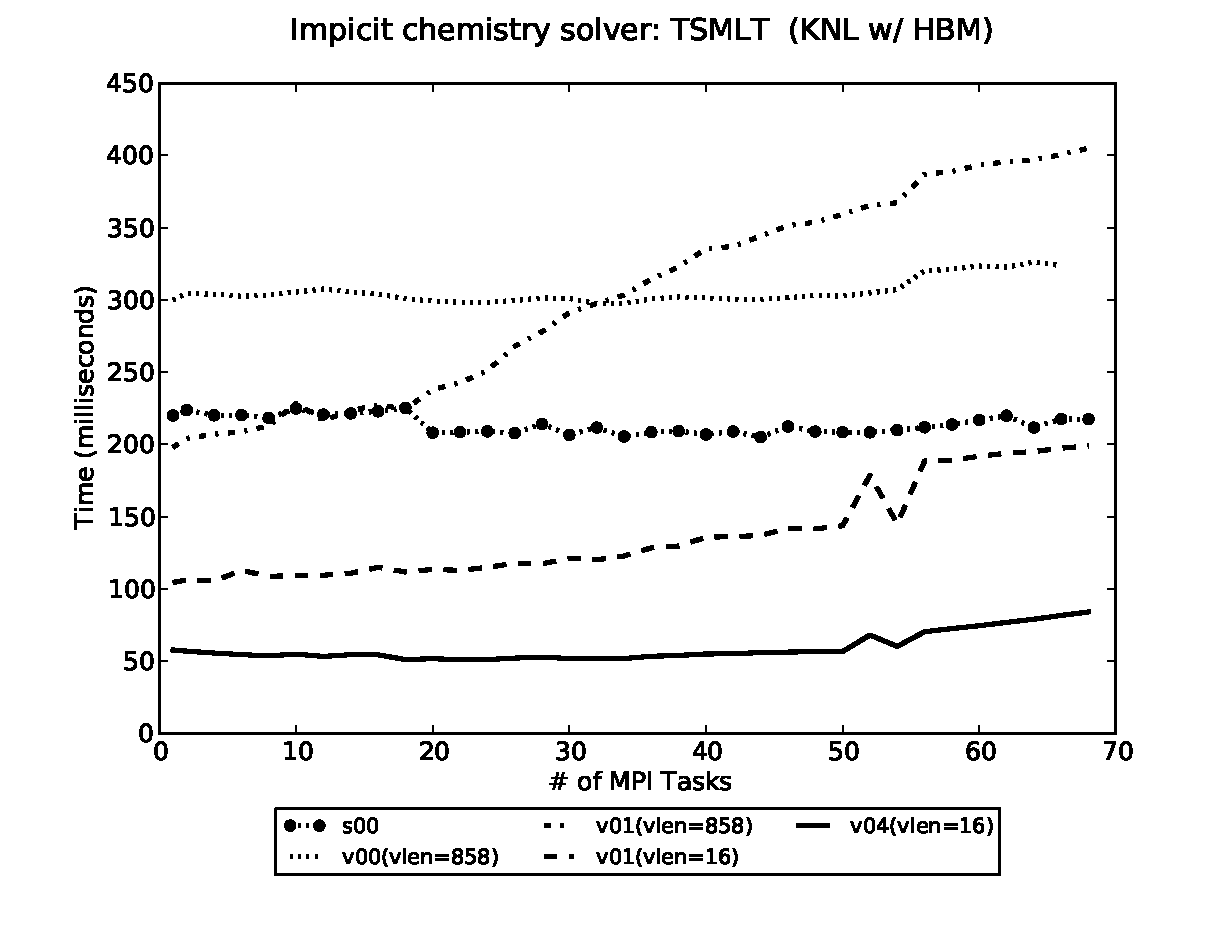
\includegraphics[width=12.0cm]{figures/chem-knl-hbm.pdf}
      \caption{Weak scaling for the implicit chemistry solver Knights Landing using high bandwidth memory in flat mode.}
      \end{center}
\end{minipage}
\end{figure}

Setting the vector length to 64 also increased the performance of the code.  This increased the performance on Sandy Bridge by about 0.5, 0.4 on Haswell, and it had little affect on the KNC.  This brought the total increase in performance to 2.35 on Sandy Bridge and 2.01 on Hawell, our target optimization amounts.  This is shown in row 6 in Table 2 (?Vector w/ Vector Length = 64?).

\begin{figure}
\centering
\begin{minipage}{1.\textwidth}
   \begin{center}
   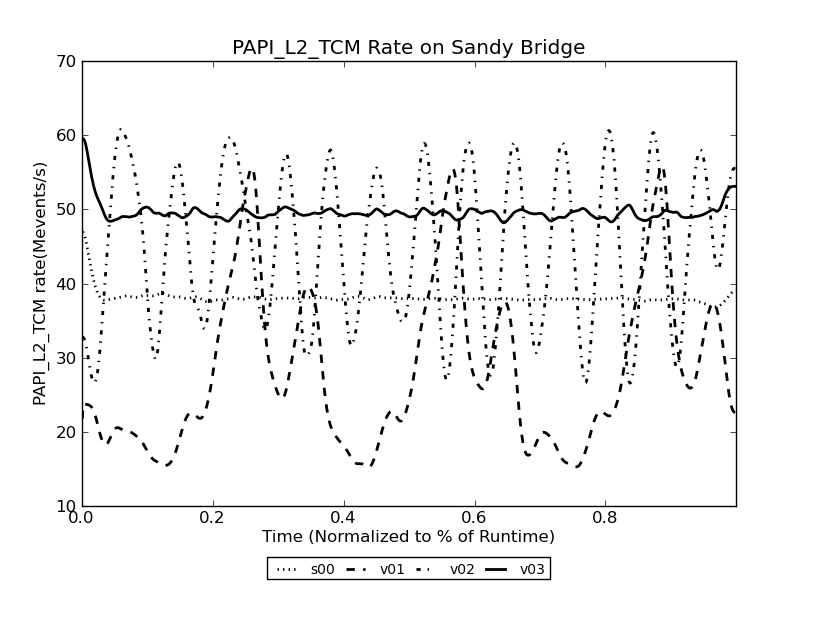
\includegraphics[width=1.\linewidth,height=7cm]{figures/chem-PAPI_L2_TCM.png}
   \caption{L2 data cache miss rate}
   \end{center}
\end{minipage}
\begin{minipage}{1.\textwidth}
   \begin{center}
   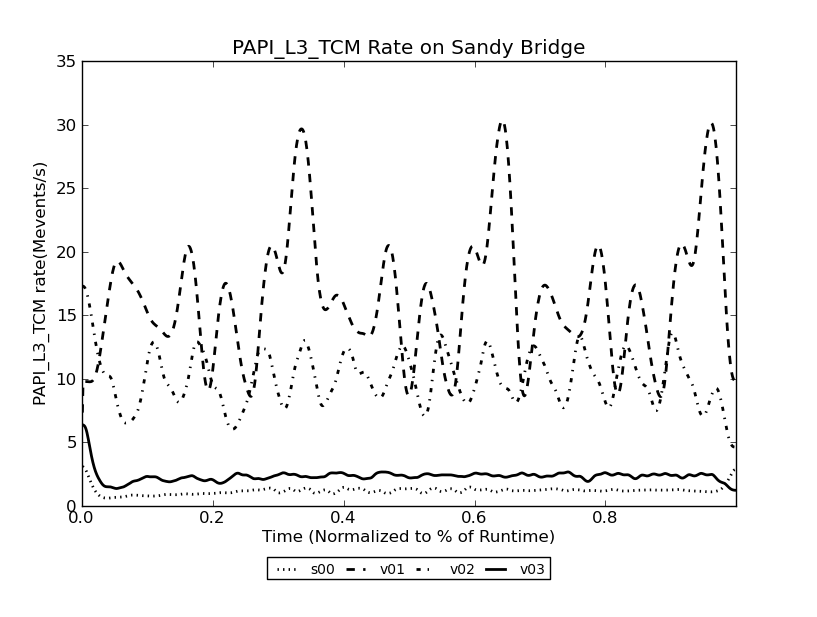
\includegraphics[width=1.\linewidth,height=7cm]{figures/chem-PAPI_L3_TCM.png}
   \caption{L3 data cache miss rate}
   \end{center}
\end{minipage}
\begin{minipage}{1.\textwidth}
   \begin{center}
   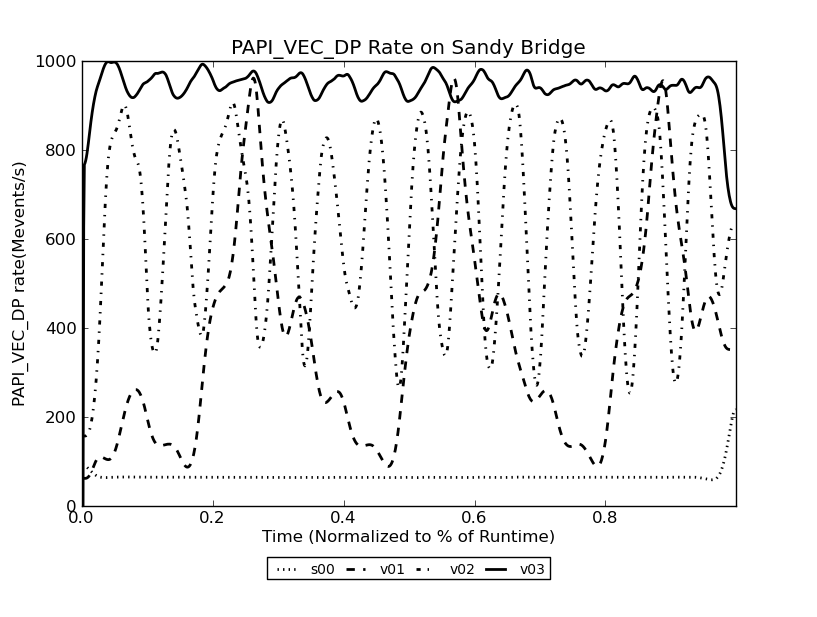
\includegraphics[width=1.\linewidth,height=7cm]{figures/chem-PAPI_VEC_DP.png}
   \caption{8-byte real vector instruction rate.}
   \end{center}
\end{minipage}
\end{figure}





